\pdfminorversion=7
\PassOptionsToPackage{obeyspaces}{url}
\documentclass[latin1, english, usepdftitle=false, svgnames, color="table, fixpdftex, fixinclude, xcdraw", t]{beamer}


\usepackage{latexscholar-i18n}
\usepackage{latexscholar-verbatim}
\usepackage{lode-imacid}
\usepackage{latexscholar-pdf}

\usepackage{animate}

\usepackage{inputx}
\inputpaths{../CommonAssets/}
\graphicspath{{../CommonAssets/figs/}}

\title{Software testing}
\subtitle{Basic concepts}
\author[]{%
	Marco Aur�lio Graciotto Silva\inst{1}, \and
	Ellen Francine Barbosa\inst{2}, \\\and
	Jos� Carlos Maldonado\inst{2}
}

\newcommand{\numberofinstitutes}{2}
\institute[ICMC]
{
	\inst{1}%
	\textbf{Department of Computing}\\
	Federal University of Technology -- Paran� (UTFPR)\\
	Campo Mour�o, PR, Brazil
	\and
	\inst{2}%
	\textbf{Institute of Mathematical Sciences and Computing}\\
	University of S�o Paulo (USP)\\
	S�o Carlos, SP, Brazil
	
}

\date[]{2017}

\logopicture{icmc-qualipso-inf}

\begin{document}

\frontmatter{}
\begin{frame}[c, plain]
\label{title}
\titlepage
\end{frame}

%\begin{frame}[c,parent={title}, hasprev=false, hasnext=false]
%\frametitle{Software Testing}
%\label{cmap:software-testing}
%
%\insertcmap{Courses-SoftwareTesting-SoftwareTesting}
%\end{frame}

\begin{frame}[c,parent={title}, hasprev=false, hasnext=false]
\frametitle{Software Testing}
\label{cmap:software-testing}

\centering
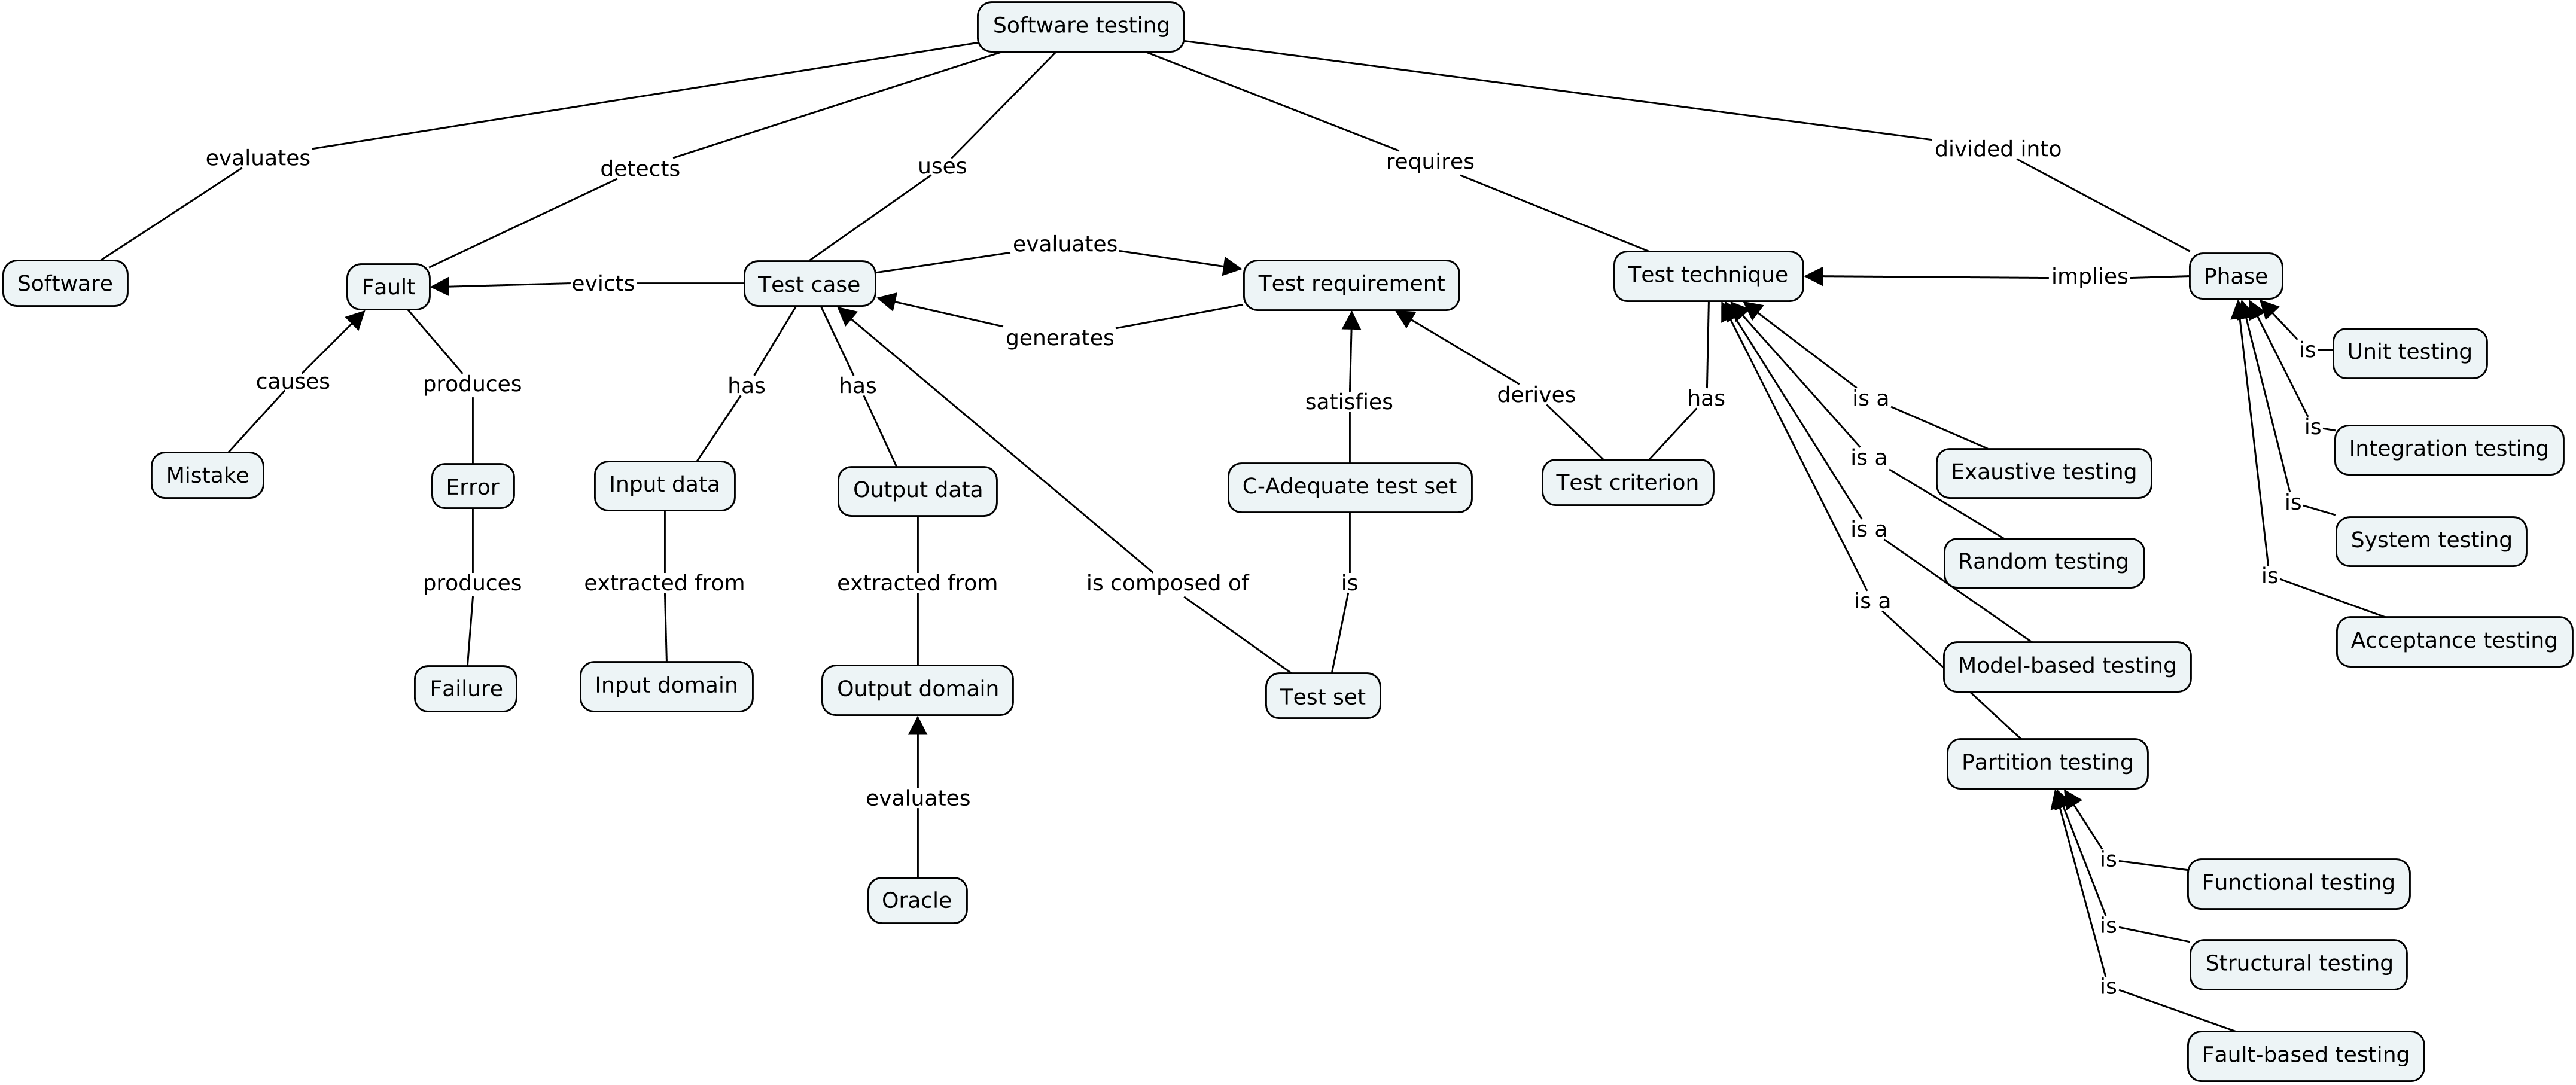
\includegraphics[width=\textwidth]{../BasicConcepts/Software testing fundamentals.png}
\end{frame}


\mainmatter{}

\part{Software Testing}
\section{Software testing}
\include{main/software-testing}

\subsection{Defect}
\include{main/software-testing/defect}

\subsection{Software testing}
\include{main/software-testing/software-testing}

\subsection{Defect taxonomy}
\include{main/software-testing/defect-taxonomy}
 
\subsection{Test case}
\begin{frame}[parent={cmap:software-testing-foundations}, hasprev=false, hasnext=true]
\frametitle{Test case}
\label{concept:test-case}
\label{concept:input-domain}
\label{concept:output-domain}
\label{concept:input-data}
\label{concept:output-data}

\begin{block:concept}{Simplified definition}
A test case is a pair consisting of test data (a set of values, one for each
input variable) to be input to the program and the expected output.
\end{block:concept}


\begin{block:concept}{A better definition}
A test case is usually defined as a tuple $(d, S(d))$, where:
\begin{itemize}
	\item $d \in D$ (and $D$ is the input domain), and
	\item $S(d)$ represents the expected output for the input $d$
	according to specification $S$.
\end{itemize}
\end{block:concept}

\hfill
\refie{example:sort-test-cases}{\beamerbutton{Example: Test cases for a sort method}}
\refie{example:num-zero-test-cases}{\beamerbutton{Example: Test cases for the numZero method}}
\end{frame}


\begin{frame}[hasprev=false, hasnext=true]
\frametitle{Test case}
\framesubtitle{Assessing a test case}
\label{concept:test-case-success}
\label{concept:test-case-failure}

\begin{block:fact}{Successful test cases}
\begin{itemize}
	\item At first, a well-constructed and executed test case is successful
	when it finds errors~\cite[p. 7]{myers:2004}

	\item It is also successful when it eventually establishes that there are
	no more errors to be found (as when applying a test criteria and satisfying
	all the test requirements).
\end{itemize}
\end{block:fact}

\begin{block:fact}{Unsuccessful test cases}
\begin{itemize}
	\item A unsuccessful test case is one that causes a program to product the
	correct result without finding any error.
\end{itemize}
\end{block:fact}

\hfill
\refie{example:doctor-laboratory-test}{\beamerbutton{Analogy for test cases success and failure}}
\end{frame}



\begin{frame}
\frametitle{Test case}

\begin{block:fact}{Execution order}
\begin{itemize}
    \item There are two styles of test case design regarding order of test
    execution:
	\begin{itemize}
		\item cascading test cases, and
		\item independent test cases.
	\end{itemize}
\end{itemize}
\end{block:fact}
\end{frame}


\begin{frame}
\label{concept:cascading-test-case}
\frametitle{Test case}
\framesubtitle{Cascading test case}

\begin{block:concept}{Definition}
Cascading test cases are test cases that build on each other.
\end{block:concept}


\begin{block:fact}{Advantages and disadvantages}
\begin{itemize}
	\item The advantage of cascading test cases is that each test case is
	typically small and simple.

	\item The disadvantage of cascading test cases is that if one test fails,
	the subsequent tests may be invalid.
\end{itemize}
\end{block:fact}

\hfill
\refie{example:cascading-test-case}{\beamerbutton{Example: Cascading test cases}}
\end{frame}



\begin{frame}[hasprev=true, hasnext=false]
\label{concept:independent-test-case}
\frametitle{Test case}
\framesubtitle{Independent test case}

\begin{block:concept}{Definition}
Independent test cases are entirely self contained.
\begin{itemize}
	\item Independent test cases neither build on each other nor require that
	other tests have been successfully executed.
\end{itemize}
\end{block:concept}

\begin{block:fact}{Advantages and disadvantages}
\begin{itemize}
	\item The advantage of independent test cases is that any number of tests
	can be executed in any order.

	\item The disadvantage of independent test cases is that each test tends to
	be larger and more complex and thus more difficult to design, create, and
	maintain.
\end{itemize}
\end{block:fact}
\end{frame}

\subsection{Oracle}
\include{main/software-testing/oracle}

\subsection{Test phase}
\begin{frame}[parent={cmap:software-testing-foundations}, hasprev=false, hasnext=true]
\frametitle{Test phases}

\begin{block:fact}{What I should test first?}
\begin{itemize}
	\item What should I target when testing a software?

	\item The definition of a single target for each test activity is key for
	systematic software testing.
	\begin{itemize}
		\item Focus effort and restrict available techniques (thus lowering
		costs and, probably, increasing efficacy).
	\end{itemize}

	\item A common sense approach would be to begin testing the smallest
	module possible, and then proceed to test the interactions between these
	modules and, finally, the system as a whole.
\end{itemize}
\end{block:fact}
\end{frame}


\begin{frame}[hasprev=true, hasnext=true]
\frametitle{Test phases}
\label{concept:test-phase}
\label{concept:phase}

\begin{block:concept}{Definition}
Test phase is a categorization of test activities which is directly related
to the software life cycle the activities take place in.
\end{block:concept}

\begin{block:fact}{Definitions}
\begin{itemize}
	\item Test phases allow the tester to concentrate on various aspects of
	the software and use different test criteria at each one.

	\item Test activities are organized in test phases such that testing starts
	with the smallest executable unit until reaching the software as a whole:
	\begin{itemize}
		\item Unit testing.
		\item Integration testing.
		\item System testing.
		\item Acceptance testing.
	\end{itemize}
\end{itemize}
\end{block:fact}
\end{frame}


\begin{frame}[c]
\frametitle{Test phases}

\begin{block:fact}{}
    \centering
    \includegraphics[scale=.3]{test-phases}
\end{block:fact}
\end{frame}


\begin{frame}
\frametitle{Test phases}
\framesubtitle{Unit testing}
\label{concept:unit-testing}

\begin{block:concept}{Definition}
Unit testing verifies the functioning in isolation of software pieces which
are separately testable.
\end{block:concept}

\begin{block:fact}{}
    \centering
    \includegraphics[width=5cm]{unit-testing}
\end{block:fact}

\hfill
\refie{example:pentium-fdiv-bug}{\beamerbutton{Example: Pentium FDIV bug}}
\end{frame}


\begin{frame}
\frametitle{Test phases}
\framesubtitle{Unit testing}

\begin{block:fact}{What is an unit?}
\begin{itemize}
	\item In procedural testing, the unit is the procedure or subroutine.

	\item In object oriented testing, the unit is the method or the class.
	\begin{itemize}
		\item For the time being, we will consider that the unit is the method!
	\end{itemize}
\end{itemize}
\end{block:fact}
\end{frame}



\begin{frame}
\frametitle{Test phases}
\framesubtitle{Unit testing - Stubs}

\begin{block:fact}{How to test an unit?}
\begin{itemize}
	\item Although the definition calls for units that are separately testable,
	this is not always possible.
	\begin{itemize}
		\item Mosts units requires data from other units.
	\end{itemize}

	\item Coupling between units is a threat for unit testing. Thus, it is
	desirable to replace some units by others more simple and predictable
	(just for software testing sake).
\end{itemize}
\end{block:fact}
\end{frame}



\begin{frame}
\frametitle{Test phases}
\framesubtitle{Stubs}
\label{concept:stub}

\begin{block:concept}{Definition}
A stub is a unit that replaces another unit used by the unit under test.
\end{block:concept}

\begin{block:fact}{Why should we use a stub?}
\begin{itemize}
	\item Stubs simulate the behavior of another unit not yet implemented but
	called by the unit under test.

	\item Usually, a stub simulates the expected behavior of the used unit with
	minimum computation effort or data manipulation.
\end{itemize}
\end{block:fact}

\hfill
\refie{example:stub}{\beamerbutton{Example: Stub}}
\end{frame}


\begin{frame}
\frametitle{Test phases}
\framesubtitle{Unit testing - Driver}

\begin{block:fact}{How to test a unit?}
\begin{itemize}
	\item Even though stubs can be used to replace complex units for a given
	unit under testing, something must setup and wire the stubs into the
	unit.
\end{itemize}
\end{block:fact}
\end{frame}



\begin{frame}
\frametitle{Test phases}
\framesubtitle{Unit testing - Driver}
\label{concept:driver}
\label{concept:test-driver}

\begin{block:concept}{Definition}
Driver is the software responsible for coordinating the testing of a unit.
\end{block:concept}

\begin{block:fact}{What a driver does?}
\begin{itemize}
	\item Drivers are used to test a unit which requires input data provided
	by another unit:
	\begin{enumerate}
		\item it gathers the data provided by the tester,
		\item it passes them to the unit under test in the form of arguments,
		\item it collects the results produced by the unit, and
		\item it shows them to the tester.
	\end{enumerate}
\end{itemize}
\end{block:fact}
\end{frame}


\begin{frame}[c]
\frametitle{Test phases}
\framesubtitle{Unit testing - Driver and stubs}

\begin{block:fact}{}
	\centering
	\includegraphics[scale=.3]{driver-and-stub}
\end{block:fact}
\end{frame}



\begin{frame}
\label{concept:integration-testing}
\frametitle{Test phases}
\framesubtitle{Integration testing}

\begin{block:concept}{Definition}
Integration testing verifies whether the units tested individually communicate
accordingly when integrated.
\end{block:concept}

\begin{block:fact}{}
    \centering
    \includegraphics[scale=.3]{integration-testing}
\end{block:fact}

\hfill
\refie{example:mars-climate-orbiter}{\beamerbutton{Example: Mars climate orbiter}}
\end{frame}



\begin{frame}
\frametitle{Test phases}
\framesubtitle{Integration testing}

\begin{block:fact}{Why integration testing is important?}
\begin{itemize}
	\item Integration testing must be performed because:
	\begin{itemize}
		\item Data can be lost at the unit's interface.

		\item Global variables can suffer undesirable interferences.
	\end{itemize}
\end{itemize}
\end{block:fact}

\begin{block:fact}{}
    \centering
    \includegraphics[width=\textwidth]{types-integration-errors}
\end{block:fact}
\end{frame}


\begin{frame}
\label{concept:system-testing}
\frametitle{Test phases}
\framesubtitle{System testing}

\begin{block:concept}{Definition}
System testing ensures that the software and the other elements that
are part of the system (hardware and database, for instance) are adequately
combined and behave as expected.
\end{block:concept}

\begin{block:fact}{Types of system testing}
\begin{itemize}
	\item Typically system testing includes many types of testing:
	\begin{columns}[t, totalwidth=6.5cm]
		\begin{column}[t]{3cm}
			\begin{itemize}
				\item functionality,
				\item usability,
				\item security,
				\item localization,
			\end{itemize}
		\end{column}

		\begin{column}[t]{3cm}
			\begin{itemize}
				\item reliability,
				\item availability,
				\item \ldots
			\end{itemize}
		\end{column}
	\end{columns}
\end{itemize}
\end{block:fact}

\hfill
\refie{example:ghost-train}{\beamerbutton{Example: Ghost train}}
\end{frame}



\begin{frame}[hasprev=true, hasnext=false]
\label{concept:acceptance-testing}
\frametitle{Test phases}
\framesubtitle{Acceptance testing}

\begin{block:concept}{Definition}
Acceptance testing refers to the tester, in general performed by the
user himself, who verifies whether the product satisfies his expectation.
\end{block:concept}

\begin{block:fact}{Alpha/Beta testing}
\begin{itemize}
	\item Informally, it can be defined alpha and beta testing.
	\begin{itemize}
		\item Alpha testing: software is installed and used internally (in the
		company that developed).

		\item Beta testing: software is installed and tested by external
		users.
	\end{itemize}
\end{itemize}
\end{block:fact}

\begin{block:fact}{Why is acceptance testing important?}
\begin{itemize}
    \item Acceptance testing, when completed successfully, will result in the
    customer accepting the software.
\end{itemize}
\end{block:fact}
\end{frame}

\subsection{Test criterion}
\begin{frame}[hasprev=false, hasnext=true]
\label{example:test-criterion}
\frametitle{Test criterion example}

\begin{itemize}
	\item Suppose we are given the enviable task of testing bags of jelly beans.
	We need to come up with ways to sample from the bags.

	\item Suppose these jelly beans have the following six flavors and come in
	four colors: Lemon (colored Yellow), Pistachio (Green), Cantaloupe (Orange),
	Pear (White), Tangerine (also Orange), and Apricot (also Yellow).

	\item A simple approach to testing might be to test one jelly bean of each
	flavor. Then we have six test requirements, one for each flavor.

	\item We satisfy the test requirement ``Lemon'' by selecting and, of course,
	tasting a Lemon jelly bean from a bag of jelly beans.
\end{itemize}
\end{frame}


\begin{frame}[hasprev=true, hasnext=false]
\frametitle{Test criterion example}

\begin{itemize}
	\item The ``flavor criterion'' yields a simple strategy for selecting jelly
	beans.

	\item In this case, the set of test requirements, $TR$, can be formally
	written out as \foreign{TR = \{flavor = Lemon, flavor = Pistachio,
	flavor = Cantaloupe, flavor = Pear, flavor = Tangerine, flavor = Apricot\}}.
\end{itemize}
\end{frame}




\subsection{Test requirement}
\include{main/software-testing/test-requirement}

\subsection{Test technique}
\begin{frame}[parent={cmap:software-testing-foundations}, hasprev=false, hasnext=true]
\frametitle{Test technique}
\label{concept:test-technique}

\begin{block:concept}{Definition}
Test techniques are types of testing defined according to the
source of information used to carried out the testing activity.
\end{block:concept}

\begin{block:fact}{Test techniques and test criteria}
\begin{itemize}
    \item Each test technique has a set of associated test criteria.
\end{itemize}
\end{block:fact}
\end{frame}



\begin{frame}[hasprev=true, hasnext=true]
\frametitle{Test technique}

\begin{block:fact}{Software test techniques}
\begin{itemize}
	\item Exhaustive testing

	\item Random testing

	\item Partition testing
	\begin{itemize}
		\item Fault-based testing

		\item Functional testing

		\item Structural testing
	\end{itemize}
\end{itemize}
\end{block:fact}
\end{frame}



\begin{frame}
\frametitle{Test technique}
\framesubtitle{Exhaustive testing}
\label{concept:exhaustive-testing}

\begin{block:concept}{Definition}
An exhaustive test executes the software with all possible value from its
input domains.
\end{block:concept}

\begin{block:fact}{}
    \centering
    \includegraphics[width=\textwidth]{exhaustive-software-testing}
\end{block:fact}

\hfill
\refie{example:blech-exhaustive-testing}{\beamerbutton{Example: Exhaustive testing of the blech function}}
\end{frame}



\begin{frame}
\frametitle{Test technique}
\framesubtitle{Exhaustive testing}

\begin{block:fact}{Exhaustive testing limitations}
\begin{itemize}
	\item Can be prohibitive due to time and cost constraints for finite
	but large input domain.

	\item Impossible if the input domain is infinite.

	\item Infeasible in general.
\end{itemize}
\end{block:fact}
\end{frame}



\begin{frame}
\frametitle{Test technique}
\framesubtitle{Random testing}
\label{concept:random-testing}

\begin{block:concept}{Definition}
Random testing uses a systematic method to generate test cases: it
requires modeling the input space and then sampling data from the input
space randomly.
\end{block:concept}

\begin{block:fact}{}
    \centering
    \includegraphics[width=\textwidth]{random-software-testing}
\end{block:fact}
\end{frame}


\begin{frame}
\frametitle{Test technique}
\framesubtitle{Random testing}

\begin{block:concept}{Reliability}
\begin{itemize}
	\item Using random testing, statistical measures of reliability can be
	achieved according to an operational profile.

	\item For every (input data of a) test case, it is assigned a probability
	distribution according to their occurrence in actual operation.
\end{itemize}
\end{block:concept}

\begin{block:fact}{Effectiveness}
\begin{itemize}
	\item It depends on the correctly definition of the operational profile.

	\item If the probability of occurrence of each input data is the same,
	random testing is regarded as the least effective technique for software
	testing~\cite[p. 43]{myers:2004}.
\end{itemize}

\end{block:fact}


\end{frame}


\begin{frame}
\frametitle{Test technique}
\framesubtitle{Partition testing}
\label{concept:partition-testing}

\begin{block:concept}{Definition}
Partition testing is meant as any testing scheme which forces execution
of at least one test case from each subset of a partition of the input
domain.
\end{block:concept}

\begin{block:fact}{}
    \centering
    \includegraphics[width=\textwidth]{partition-software-testing}
\end{block:fact}
\end{frame}



\begin{frame}
\frametitle{Test technique}
\framesubtitle{Functional testing}
\label{concept:functional-testing}

\begin{block:concept}{Definition}
Functional testing is a technique based solely on the requirements and
specifications.
\end{block:concept}

\begin{block:fact}{}
\begin{itemize}
	\item Functional testing is also known as black box testing.

	\item Functional testing obtains test requirements from the
	software specification.
	\begin{itemize}
		\item Functional testing requires no knowledge of the internal paths,
		structure, or implementation of the software under test.
	\end{itemize}
\end{itemize}
\end{block:fact}

\hfill
\refie{example:functional-testing}{\beamerbutton{Example}}
\end{frame}


\begin{frame}
\frametitle{Test technique}
\framesubtitle{Functional testing}

\begin{block:fact}{Functional test criteria}
\begin{itemize}
	\item Equivalence partition.
	\item Boundary-value analysis.
	\item Cause-effect graph.
	\item \ldots
\end{itemize}
\end{block:fact}
\end{frame}



\begin{frame}
\frametitle{Test technique}
\framesubtitle{Structural testing}

\begin{block:concept}{Definition}
Structural testing is a technique based on the internal paths, structure,
and implementation of the software under test.
\end{block:concept}


\begin{block:fact}{}
\begin{itemize}
	\item Structural testing is also known as white box testing.

	\item Structural testing obtains test requirements from implementation
	features.
\end{itemize}
\end{block:fact}

\begin{block:fact}{}
    \centering
    \includegraphics[width=6cm]{structural-testing}
\end{block:fact}
\end{frame}


\begin{frame}
\frametitle{Test technique}
\framesubtitle{Structural testing}
\label{concept:structural-testing-criteria}

\begin{block:fact}{Control-flow based criteria}
\begin{itemize}
	\item Criteria based on the flow of control within a program:
	\begin{itemize}
		\item Statement coverage.
		\item Decision coverage.
		\item Condition coverage.
		\item \ldots
	\end{itemize}
\end{itemize}
\end{block:fact}


\begin{block:fact}{Data-flow based criteria}
\begin{itemize}
	\item Criteria based on the usage of data (variable creation, definition,
	and use):
	\begin{itemize}
		\item All-uses.
		\item All-potential-uses
		\item \ldots
	\end{itemize}
\end{itemize}
\end{block:fact}


\hfill
\refie{example:structural-testing}{\beamerbutton{Example}}
\end{frame}




\begin{frame}
\frametitle{Test technique}
\framesubtitle{Fault-based testing}
\label{concept:fault-based-testing}

\begin{block:concept}{Definition}
Fault-based testing is a technique in which testing is based on
historical information about common faults detected during the software
development life cycle.
\end{block:concept}

\begin{block:fact}{}
    \centering
    \includegraphics[width=7cm]{mutation-testing}
\end{block:fact}
\end{frame}


\begin{frame}[hasprev=true, hasnext=false]
\frametitle{Test technique}
\framesubtitle{Fault-based testing}
\label{concept:fault-based-test-criteria}

\begin{block:fact}{Fault-based test criteria}
\begin{itemize}
	\item Error seeding.
	\item Mutation:
	\begin{itemize}
		\item Mutation analysis.
		\item Interface mutation.
		\item \ldots
	\end{itemize}
\end{itemize}
\end{block:fact}

\hfill
\refie{example:fault-based-testing}{\beamerbutton{Example}}
\end{frame}


\subsection{Software testing process}
\include{main/software-testing/software-testing-process}


\part{References and credits}
\backmatter{}
\include{bibliography}
\part{Acknowledgement}
\section*{Acknowledgement}


\begin{frame}[c,label=credits]
\frametitle{Credits}

\centering
\animategraphics[height=140pt,poster=first,autoplay,loop]{1}{main/jabuti-}{0}{3}

\begin{itemize}
	\item Reviewers:
	\begin{itemize}
		% \item Auri Marcelo Rizzo Vincenzi
		% \item Ellen Francine Barbosa
		\item Fabiano Cutigi Ferrari
		% \item Márcio Eduardo Delamaro
		\item Otávio Augusto Lazzarini Lemos
	\end{itemize}
\end{itemize}
\end{frame}



\part{Instructional elements}
\include{examples}
\include{exercises}

\end{document}
